\normaltrue \difficilefalse \tdifficilefalse
\correctionfalse

%\UPSTIidClasse{11} % 11 sup, 12 spé
%\newcommand{\UPSTIidClasse}{11}

\exer{Véhicule à trois roues Clever$\star$ \label{B2:07:80}}

% Concours Banque PT SIA -  2011

\setcounter{question}{0}\UPSTIcompetence[2]{B2-07}
\index{Compétence B2-07}
\index{Schéma-blocs}
\index{Clever}
\ifcorrection
\else
\textbf{Pas de corrigé pour cet exercice.}
\fi

\ifprof
\else
\section*{Présentation du système}

Le Clever est un démonstrateur technologique développé par un tissu d'industriels européens. Clever est la contraction de Compact Low Emission VEhiclefor uRban tRansportation (véhicule compacte à faibles émissions pour le transport urbain) car, avec une consommation de seulement \SI{2,5}{L}/\SI{100}{km}, il s'annonce très écologique. 

L'habitacle peut s'incliner grâce à un système constitué 
\begin{itemize}
\item d'un calculateur qui détermine le mouvement et la position à donner à l'habitacle en fonction des conditions d'utilisation ;
\item d'un système hydro-mécanique de transmission de puissance et d'adaptation de mouvement ;
\item d'un système de contrôle de l'inclinaison de l'habitacle.
\end{itemize}

\begin{center}
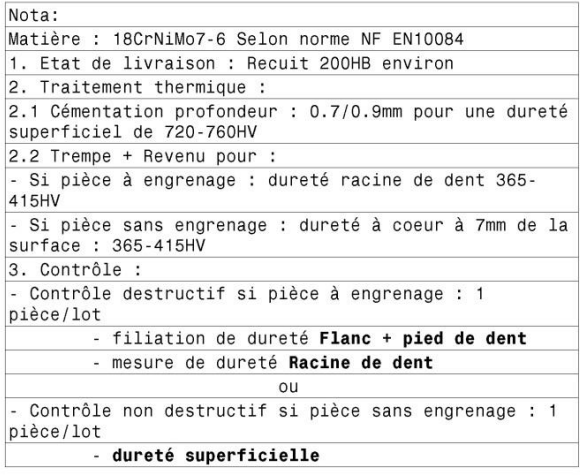
\includegraphics[width=.47\linewidth]{fig_02}
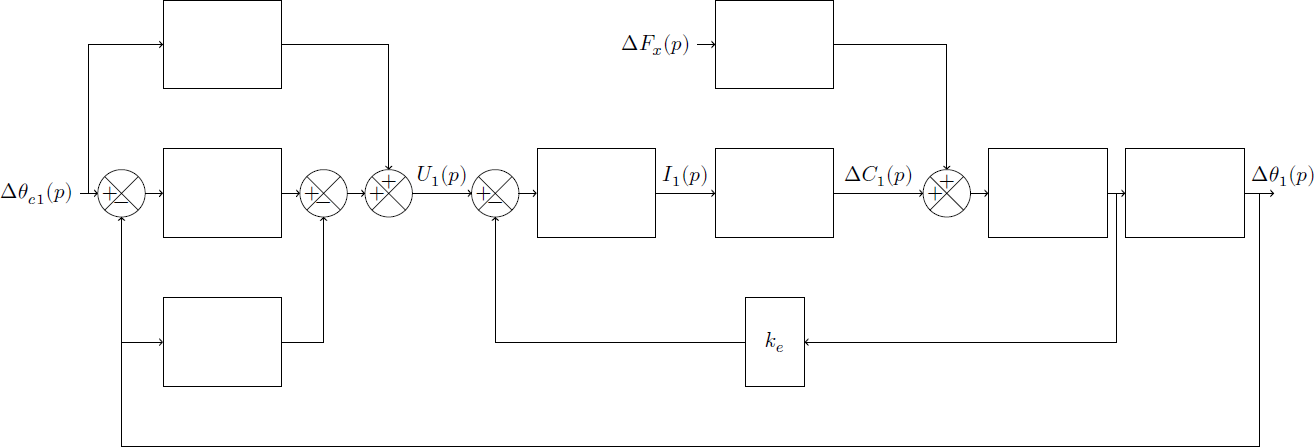
\includegraphics[width=.47\linewidth]{fig_03}
%\textit{}
\end{center}

%La chaîne de transmission de puissance et d'adaptation de mouvement est composée :
%\begin{itemize}
%\item d'une pompe à engrenages actionnée par le moteur à gaz via un système de poulies/courroie ;
%\item d'un circuit hydraulique ;
%\item de 2 vérins hydrauliques simple effet ;
%\item d'un système mécanique d'adaptation de mouvement afin de transformer le mouvement de translation des tiges des vérins en rotation de l'habitacle.
%\end{itemize}
\begin{obj}
L'objectif est que le mouvement de l'habitacle soit contrôlé :
\begin{itemize}
\item écart statique : 0\degres;
\item écart de traînage pour une entrée en rampe unitaire : 0\degres;
\item temps de réponse à 5\% : inférieur à \SI{0,1}{s}.

\end{itemize}
\end{obj}

\subsection*{Modélisation du servo-distributeur et du vérin}

L'orientation de l'habitacle est contrôlée par un asservissement de la position angulaire. L'architecture de cet asservissement est représentée par le schéma-blocs de le figure suivante.

On modélise le comportement du servo-distributeur par un gain pur noté $K_s$ et le capteur par $H_c(p)=C$ avec $C=\SI{1}{V.rad^{-1}}$.  L'adaptateur mécanique a un comportement linéaire sur l'intervalle d'utilisation. On a donc $H_{\text{am}}(p)=R$ ($R=\SI{7}{rad.m^{-1}}$). Enfin, on considère que $H_r(p)=1$. 

\begin{center}
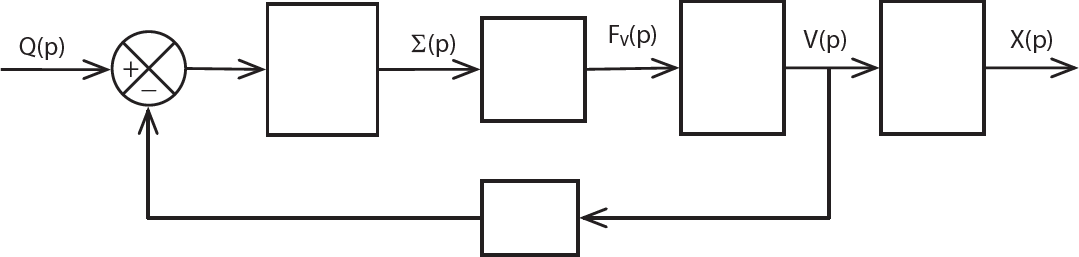
\includegraphics[width=\linewidth]{fig_05}
\end{center}

À ce stade de l'étude, le modèle de comportement du fluide correspond à un comportement incompressible. L'équation caractérisant le comportement du vérin est alors : $q(t)=S\dot{\lambda}(t)$ où :
\begin{itemize}
\item $S$ représente la section utile du vérin en sortie de tige (diamètre \SI{32}{mm});
\item $q$ est le débit en entrée de vérin ;
\item $v(t)=\dot{\lambda}(t)=\dfrac{\dd \lambda(t) }{\dd t}$ est la vitesse de translation de la tige du vérin par rapport au corps.
\end{itemize}
% 
\fi

\question{Donner l'expression de la fonction de transfert du vérin $H_{V1}(p)$ (telle que $\lambda(p) = H_{V1}(p) Q(p)$) et compléter le schéma-bloc associé à la modélisation actuelle du système.}
\ifprof
\begin{corrige} ~\\

\begin{center}
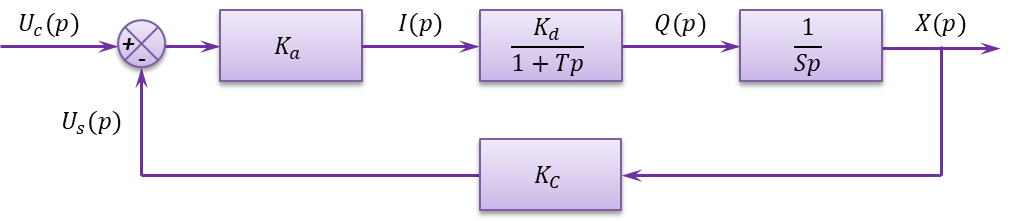
\includegraphics[width=.95\linewidth]{cor_01}
%\textit{}
\end{center}
\end{corrige}
\else
\fi

\question{Déterminer la fonction de transfert en boucle fermée $\text{FTBF}_1$ (telle que $\alpha(p) = \text{FTBF}_1(p) \alpha_c(p)$) du système bouclé. Mettre  $\text{FTBF}_1(p)$ sous la forme 
$\dfrac{K_1}{1+\tau_1 p}$ en précisant les expressions de $K_1$ et de $\tau_1$.} 
 \ifprof
\begin{corrige} ~\\

\begin{center}
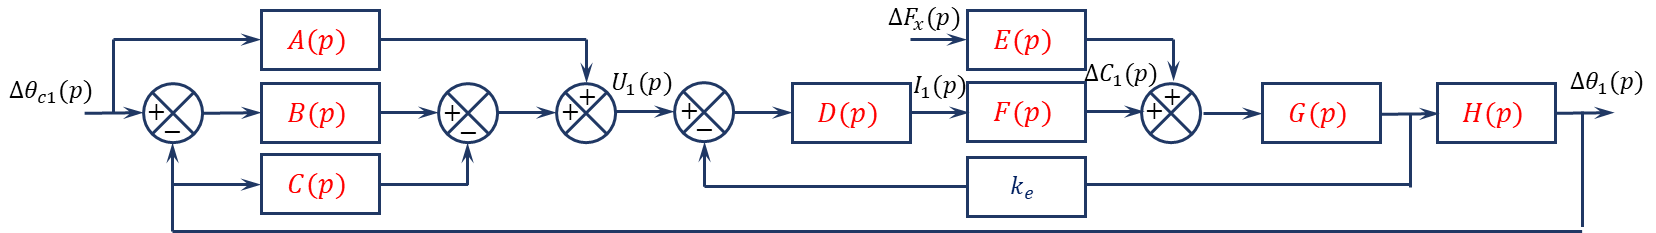
\includegraphics[width=.95\linewidth]{cor_02}
%\textit{}
\end{center}
\end{corrige}
\else
\fi


\question{ À partir du critère de temps de réponse à 5\% $(t_{r5\%})$ du système, déterminer l'expression puis la valeur numérique minimale du gain du servo-distributeur.} 

\ifprof
\begin{corrige}~\\
\begin{center}
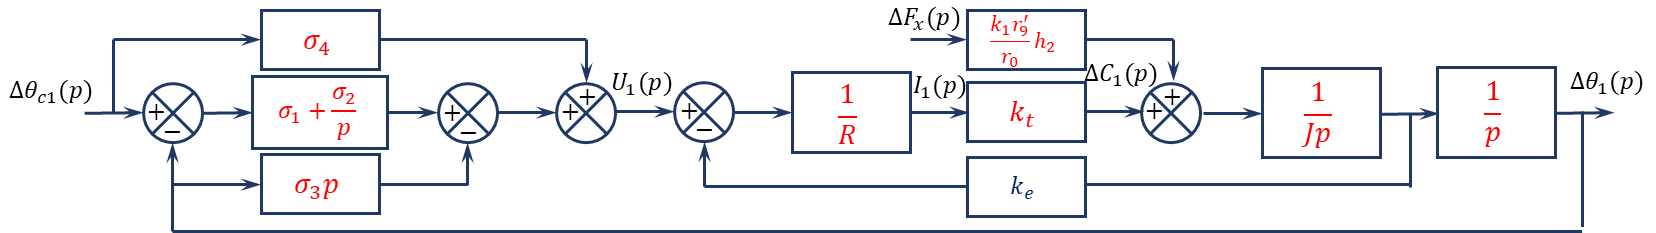
\includegraphics[width=.95\linewidth]{cor_03}
%\textit{}
\end{center}    
\end{corrige}
\else
\fi

\ifprof
\else
\subsection*{Modélisation du comportement du vérin avec fluide compressible et du comportement dynamique du mécanisme}

La compressibilité du fluide étant prise en compte dans le modèle, l'évolution du débit est une fonction du déplacement mais aussi de la pression sous la forme de la relation (1). L'effort exercé par le vérin en sortie de tige est décrit par la relation (2).
$$
q(t)=S\dot{\lambda}(t)+\dfrac{V_0}{B}\dot{p}_r(t) \quad (1) \quad\quad
F_V(t)=Sp_r(t) \quad (2)
$$
où:
\begin{itemize}
\item $p_r(t)$ : pression utile dans le vérin ;
\item $V_0$ : volume caractéristique moyen de fluide contenu dans le vérin et les durites, $V_0 = \SI{2,5e5}{m^3}$;
\item $B$ : coefficient de compressibilité du fluide, $B = \SI{109}{Pa}$;
\item $F_v(t)$ : effort développé par le vérin en sortie de tige ;
\item $S$ : section utile du vérin en sortie de tige.
\end{itemize}

Par ailleurs, $F_v(t)+k_g \lambda(t)=m_{\text{eq}}\ddot{\lambda}(t)$ avec $m_{\text{eq}}$ la masse équivalente du système, $k_g$ une constante, $\lambda(t)$ le déploiement des vérins.
\fi


\question{Appliquer la transformation de Laplace aux équations précédentes et compléter le schéma-blocs.}
\ifprof
\begin{corrige}
\begin{center}
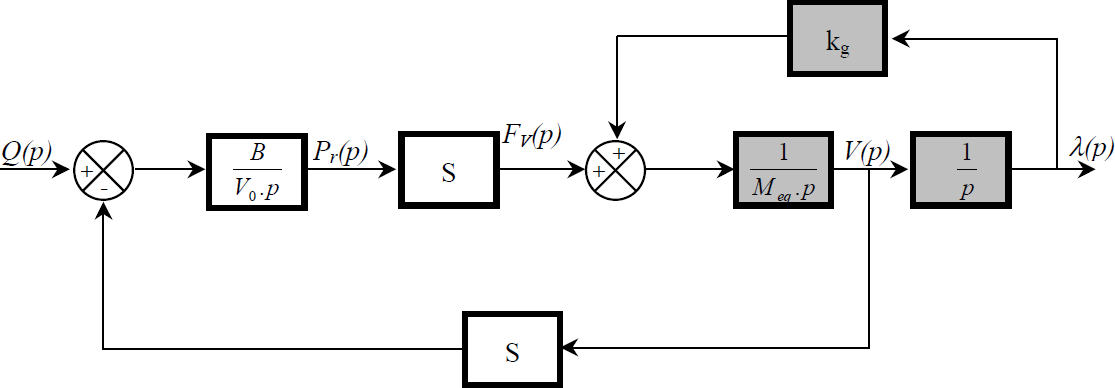
\includegraphics[width=.95\linewidth]{cor_04}
%\textit{}
\end{center}    
\end{corrige}
\else
\fi
\begin{center}
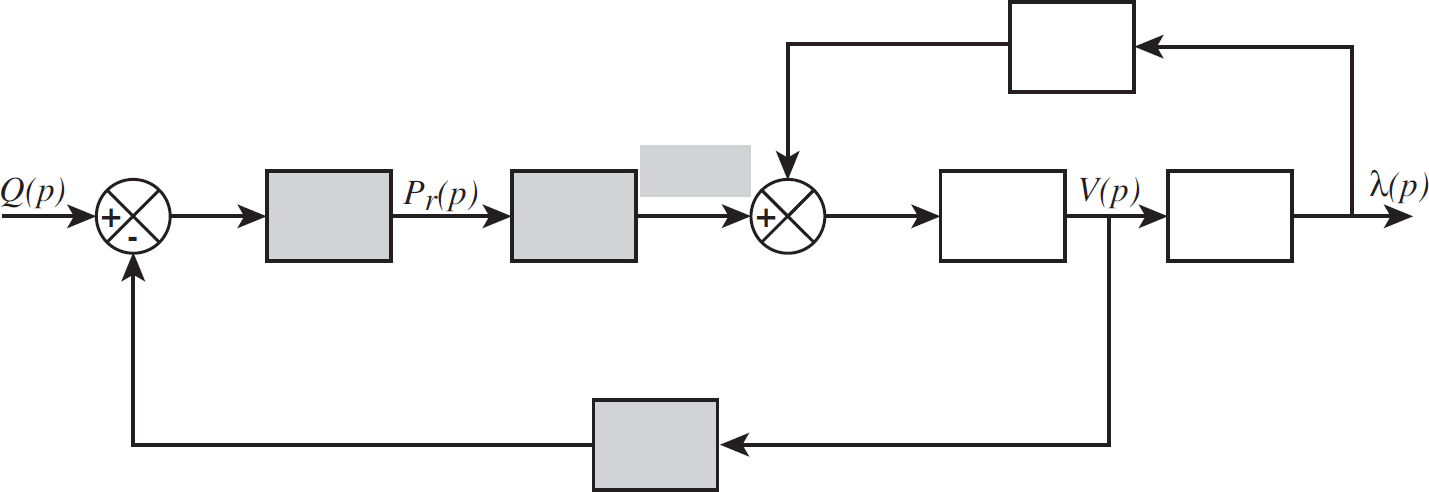
\includegraphics[width=\linewidth]{fig_06}
%\textit{}
\end{center}


\ifprof
\else
\subsection*{Analyse du comportement global}
\fi


\question{Donner l'expression de la fonction de transfert en boucle fermée du vérin $H_{\text{V2}}$ (telle que $\lambda(p) =  H_{\text{V2}} Q(p)$) et préciser les expressions des coefficients $K_V$ et $\omega_V$ de sa forme canonique : $H_{\text{V2}}(p)=\dfrac{K_V}{p\left( 1+\dfrac{p^2}{\omega_V^2}\right)}$.}
\ifprof
\begin{corrige} ~\\
\begin{center}
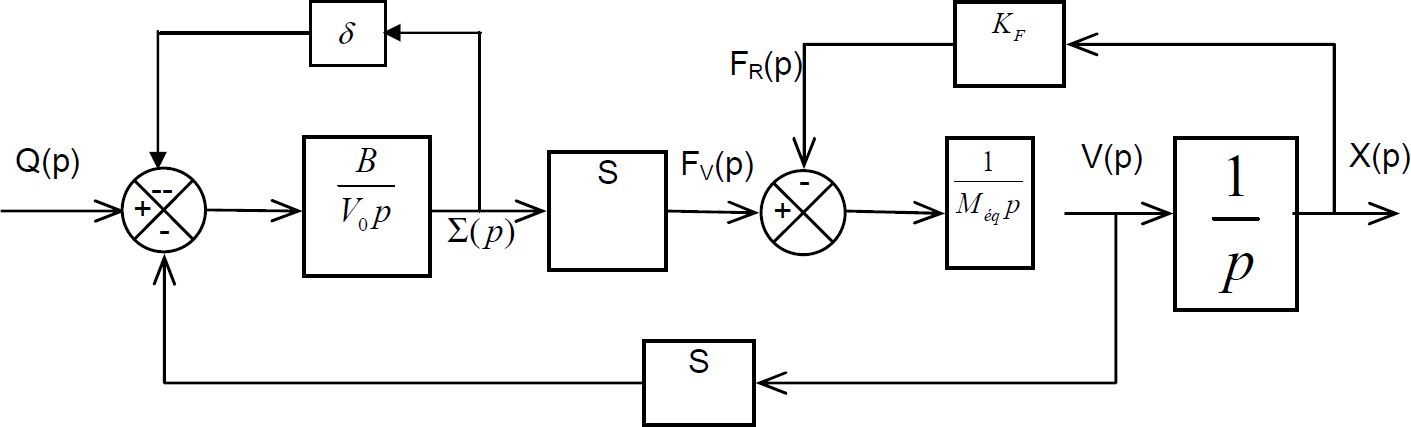
\includegraphics[width=.95\linewidth]{cor_05}
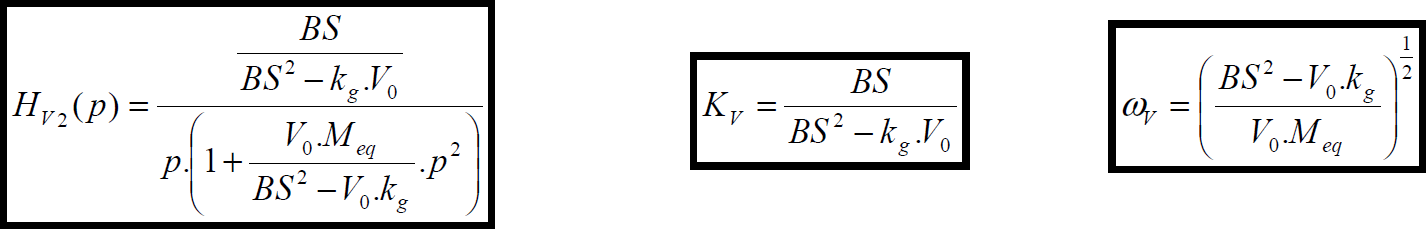
\includegraphics[width=.95\linewidth]{cor_06}
%\textit{}
\end{center}
\end{corrige}
\else
\fi


\ifprof
\else

\textbf{$k_g$ peut maintenant être négligé.}

\subsection*{Modélisation du comportement dynamique avec prise en compte d'un débit de fuite}
Pour pallier le problème de stabilité du modèle précédemment établi, une solution possible consiste à introduire un débit de fuite au niveau du vérin. Celui-ci a pour effet de réduire artificiellement le débit réel entrant dans le vérin en fonction de la pression utile. L'expression du débit est alors : 
$q(t)=S\dot{\lambda}(t)+\dfrac{V_0}{B} \dot{p}_r(t)-\delta p_r(t)$ où $\delta$ représente le coefficient de débit de fuite.
\fi


\question{Proposer une modification du schéma-bloc donné afin de prendre en compte le débit de fuite.}
\ifprof
\begin{corrige}
\begin{center}
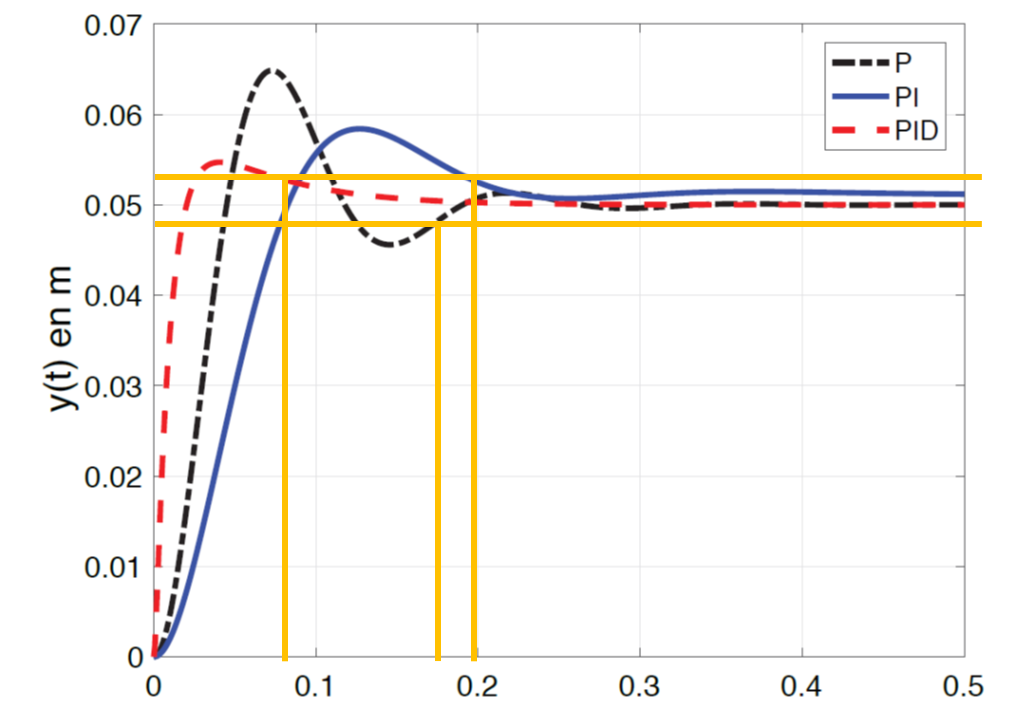
\includegraphics[width=.95\linewidth]{cor_07}
%\textit{}
\end{center}
\end{corrige}
\else
\fi
\begin{center}
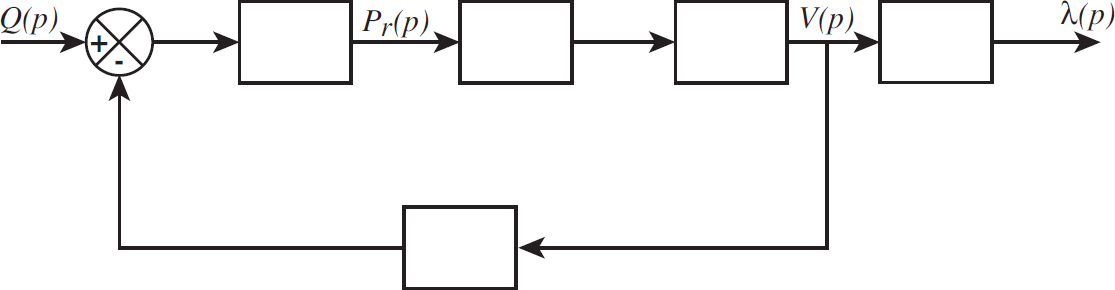
\includegraphics[width=\linewidth]{fig_08}
%\textit{}
\end{center}


\question{Déterminer l'expression de la fonction de transfert $H_{V3}$ (telle que $\lambda(p) =  H_{V3} Q(p)$) associée au comportement dynamique du vérin ainsi modélisé. On donnera le résultat sous la forme suivante : 
$H_{V3}(p)=\dfrac{K_V}{p\left(1+a_1 p + \dfrac{p^2}{\omega_V^2} \right)}$.  
Donner l'expression de $a_1$ en fonction de $M_{eq}$, $\delta$ et $S$ et déterminer l'expression du coefficient d'amortissement $\xi_V$ du second ordre en fonction de $M_{\text{eq}}$, $\delta$, $S$, $B$ et $V_0$.}
\ifprof
\begin{corrige}
\begin{center}
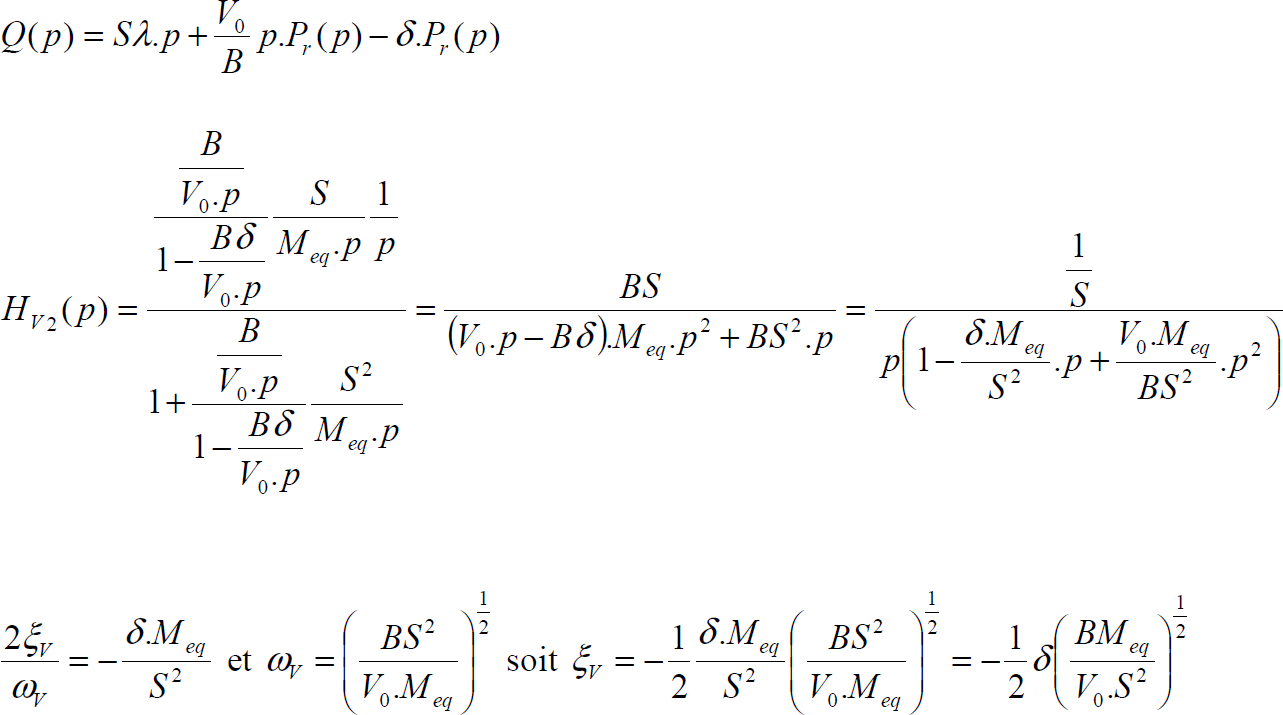
\includegraphics[width=.95\linewidth]{cor_08}
%\textit{}
\end{center}
\end{corrige}
\else
\fi

\ifprof
\else
\subsection*{Retour sur le cahier des charges}
Le régulateur étant a priori optimisé, on réalise un essai de validation du comportement temporel de l'inclinaison de l'habitacle, le véhicule étant à l'arrêt. Le calculateur envoie un signal de consigne représentant l'évolution de la position angulaire souhaitée (de 0 à 45\degres en \SI{0,75}{s}). 

\begin{center}
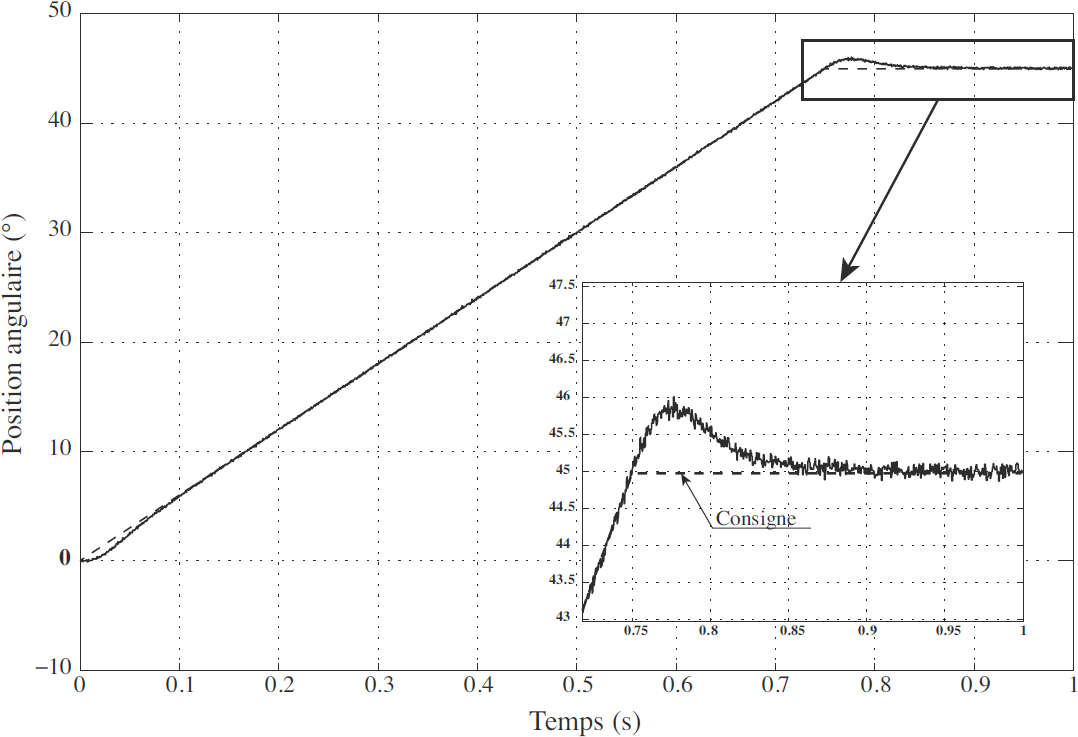
\includegraphics[width=\linewidth]{fig_09}
%\textit{}
\end{center}
\fi

\question{Quels sont les critères du cahier des charges validés ?}
\ifprof
\begin{corrige}
\begin{center}
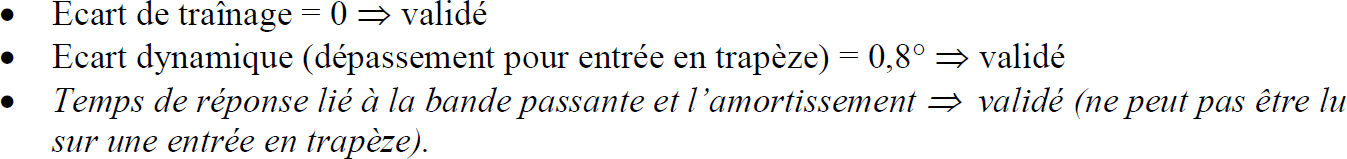
\includegraphics[width=.95\linewidth]{cor_10}
%\textit{}
\end{center}

\end{corrige}
\else
\fi



\ifprof
\else
\begin{flushright}
\footnotesize{Corrigé  voir \ref{B2:07:80}.}
\end{flushright}%
\fi